% f2015hbl_q19_pyramid.tex — 2015 年高考数学·湖北卷·理科 第 19 题（阳马）
%
% 【来源】`.work/phase3-b21/source/2015湖北理.pdf`（SHA-256
%   66e6822009bdfd8f9a5a4adf4dd3f7564fc74d8fa09906c271dc6c6a5b31a66f），
%   第 2 页（合订本页 952）；内容对象 35。逐路径实测见
%   `.work/phase3-b21/figure-inventory.md`。
%
% 【坐标口径】源 PDF 用户空间（原点左下、y 向上）。本图本地坐标
%   (x, y) = (x_page − 279.213, y_page − 196.719)，1 单位 = 1 TeX pt。
%   路径坐标逐点照录内容流（含三次贝塞尔控制点）。
%
% 元素计数：13 条路径（7 实＋6 虚）＋7 个标签
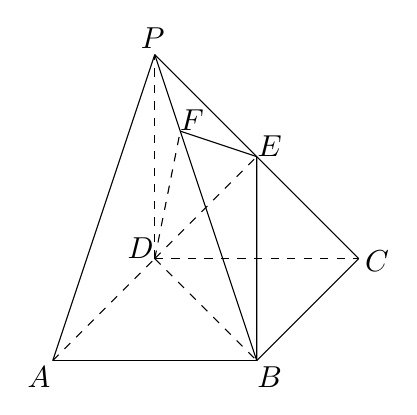
\begin{tikzpicture}[x=1pt, y=1pt,
    every node/.style={inner sep=0pt, font=\fontsize{10.5pt}{12.6pt}\selectfont}]
  \draw[line width=0.3985pt] (0.0000,0.0000)   (0.0000,0.0000)   -- (73.7162,0.0000);
  \draw[line width=0.3985pt] (73.7162,0.0000)   (73.7162,0.0000)   -- (110.5688,36.8525);
  \draw[line width=0.3985pt] (36.8525,110.5688)   (36.8525,110.5688)   -- (0.0000,0.0000);
  \draw[line width=0.3985pt] (36.8525,110.5688)   (36.8525,110.5688)   -- (73.7162,0.0000);
  \draw[line width=0.3985pt] (36.8525,110.5688)   (36.8525,110.5688)   -- (110.5688,36.8525);
  \draw[line width=0.3985pt] (73.7162,0.0000)   (73.7162,0.0000)   -- (73.7105,73.7105);
  \draw[line width=0.3985pt] (73.7105,73.7105)   (73.7105,73.7105)   -- (46.0684,82.9265);
  \draw[line width=0.3985pt, dash pattern=on 2.98883pt off 2.98883pt, dash phase=0.0pt] (0.0000,0.0000)   (0.0000,0.0000)   -- (36.8525,36.8525);
  \draw[line width=0.3985pt, dash pattern=on 2.98883pt off 2.98883pt, dash phase=0.0pt] (36.8525,36.8525)   (36.8525,36.8525)   -- (110.5688,36.8525);
  \draw[line width=0.3985pt, dash pattern=on 2.98883pt off 2.98883pt, dash phase=0.0pt] (36.8525,36.8525)   (36.8525,36.8525)   -- (36.8525,110.5688);
  \draw[line width=0.3985pt, dash pattern=on 2.98883pt off 2.98883pt, dash phase=0.0pt] (36.8525,36.8525)   (36.8525,36.8525)   -- (73.7105,73.7105);
  \draw[line width=0.3985pt, dash pattern=on 2.98883pt off 2.98883pt, dash phase=0.0pt] (36.8525,36.8525)   (36.8525,36.8525)   -- (46.0684,82.9265);
  \draw[line width=0.3985pt, dash pattern=on 2.98883pt off 2.98883pt, dash phase=0.0pt] (36.8525,36.8525)   (36.8525,36.8525)   -- (73.7162,0.0000);

  \node[anchor=center] at (36.137,116.571) {$P$};  % 源中心 (315.35,313.29)
  \node[anchor=center] at (50.287,86.921) {$F$};  % 源中心 (329.50,283.64)
  \node[anchor=center] at (78.337,77.671) {$E$};  % 源中心 (357.55,274.39)
  \node[anchor=center] at (31.737,40.821) {$D$};  % 源中心 (310.95,237.54)
  \node[anchor=center] at (117.137,35.921) {$C$};  % 源中心 (396.35,232.64)
  \node[anchor=center] at (-4.963,-5.879) {$A$};  % 源中心 (274.25,190.84)
  \node[anchor=center] at (78.387,-5.879) {$B$};  % 源中心 (357.60,190.84)

\end{tikzpicture}
%
% 【自验结果】
%   探针：latexmk -pdfxe（待跑）。
